\section{Computing continuum}

AI hardware ranges from small, low-power devices running on batteries to large-scale, high-performance systems in datacenters.
This range represents the computing continuum. 
\begin{figure}[H]
    \centering
    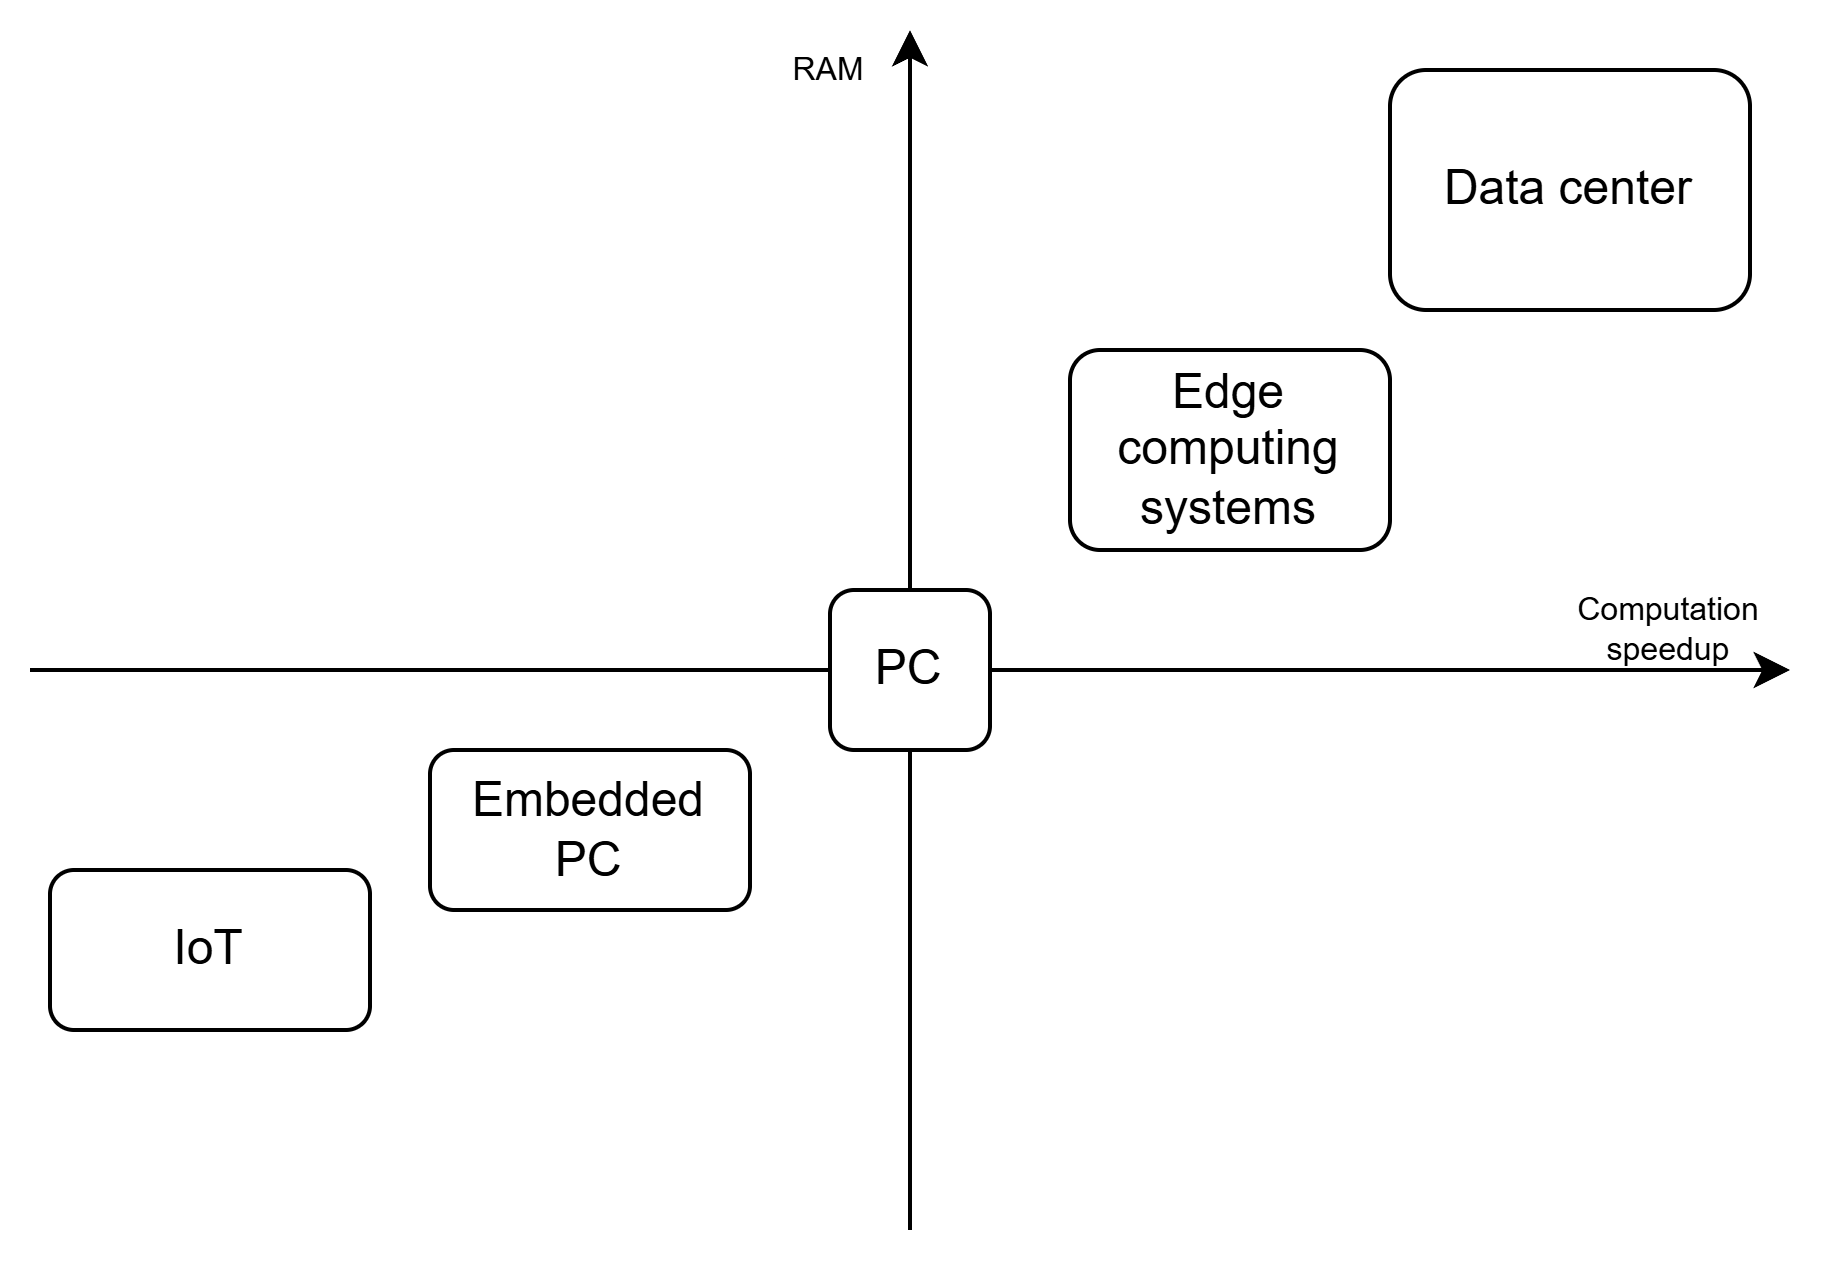
\includegraphics[width=0.5\linewidth]{images/eeai2.png}
    \caption{Computing continuum}
\end{figure}

\subsection{Datacenters}
Datacenters provide cost-efficient IT infrastructure, high-performance computing capabilities, and instant software updates.
Their vast storage capacity ensures data reliability and accessibility, allowing seamless collaboration across devices and locations. 
Furthermore, by decoupling AI processing from end-user devices, datacenters enable powerful AI applications that are not limited by local hardware constraints.

Datacenters require a constant internet connection. 
Their reliance on shared infrastructure can introduce privacy and security concerns, while the lack of direct hardware control may limit customization options. 
Additionally, the high energy consumption of large-scale AI operations raises both environmental and cost concerns. 
In latency-sensitive applications, delays in data transmission and processing can further impact real-time decision-making.

\subsection{Edge computing systems}
Edge computing delivers high computational power with the advantage of distributed processing. 
By bringing computation closer to where data is generated, it enhances privacy and security while significantly reducing latency in decision-making. 
However, these systems depend on a stable power supply and often integrate with cloud services to extend their processing capabilities.

By processing data locally, edge computing minimizes the need for constant data transmission, optimizing bandwidth and improving energy efficiency. 
This approach not only strengthens security and privacy but also enables real-time decision-making and adaptive learning across distributed networks. 
However, edge devices often operate with limited computing resources, constrained memory, and restricted energy availability. 
Their design requires careful coordination of hardware, software, and Machine Learning models, adding complexity to development and deployment.

\subsection{Embedded systems}
Embedded systems, widely used in AI applications, provide high-performance computing in a compact form. 
They benefit from the availability of development boards and can be programmed similarly to traditional computers, making them accessible to a broad community of developers. 
Despite these advantages, they tend to consume relatively high power, and in some cases, require custom hardware design to meet specific application needs.

\subsection{Internet of Things}
At the smallest scale, the Internet of Things (IoT) enables AI integration into pervasive, low-cost, battery-powered devices. 
These systems support wireless connectivity and often include sensing and actuating capabilities, making them essential for smart environments. 
However, IoT devices face limitations in computing power, energy efficiency, and memory capacity, which can complicate programming and constrain their ability to run advanced AI models.